\documentclass[onecolumn, draftclsnofoot,10pt, compsoc]{IEEEtran}
\usepackage{graphicx}
\usepackage{url}
\usepackage{setspace}

\usepackage{geometry}
\geometry{textheight=9.5in, textwidth=7in}

% 1. Fill in these details
\def \CapstoneTeamName{		Inferno}
\def \CapstoneTeamNumber{		43}
\def \GroupMemberOne{			Dennie Devito}
\def \GroupMemberTwo{			Logan Kling}
\def \GroupMemberThree{			Dakota Zaengle}
\def \CapstoneProjectName{		Solar Car Simulation}
\def \CapstoneSponsorCompany{	Phoenix Solar Racing}
\def \CapstoneSponsorPerson{		Cailin Moore}

% 2. Uncomment the appropriate line below so that the document type works
\def \DocType{		%Problem Statement
				Requirements Document
				%Technology Review
				%Design Document
				%Progress Report
				}
			
\newcommand{\NameSigPair}[1]{\par
\makebox[2.75in][r]{#1} \hfil 	\makebox[3.25in]{\makebox[2.25in]{\hrulefill} \hfill		\makebox[.75in]{\hrulefill}}
\par\vspace{-12pt} \textit{\tiny\noindent
\makebox[2.75in]{} \hfil		\makebox[3.25in]{\makebox[2.25in][r]{Signature} \hfill	\makebox[.75in][r]{Date}}}}
% 3. If the document is not to be signed, uncomment the RENEWcommand below
\renewcommand{\NameSigPair}[1]{#1}

%%%%%%%%%%%%%%%%%%%%%%%%%%%%%%%%%%%%%%%
\begin{document}
\begin{singlespace}
\begin{titlepage}
    \pagenumbering{gobble}
    \begin{singlespace}
    	%
\includegraphics[height=4cm]{Shirt_Graphic}
        \hfill
        \begin{flushleft}
        % 4. If you have a logo, use this includegraphics command to put it on the coversheet.
        
\includegraphics[height=5cm]{Shirt_Graphic.png}
        \end{flushleft}
        \par\vspace{.2in}
        \centering
        \scshape{
            \huge CS Capstone \DocType \par
            {\large\today}\par
            \vspace{.5in}
            \textbf{\Huge\CapstoneProjectName}\par
            \vfill
            {\large Prepared for}\par
            \Huge \CapstoneSponsorCompany\par
            \vspace{5pt}
            {\Large\NameSigPair{\CapstoneSponsorPerson}\par}
            {\large Prepared by }\par
            Group\CapstoneTeamNumber\par
            % 5. comment out the line below this one if you do not wish to name your team
            \CapstoneTeamName\par 
            \vspace{5pt}
            {\Large
                \NameSigPair{\GroupMemberOne}\par
                \NameSigPair{\GroupMemberTwo}\par
                \NameSigPair{\GroupMemberThree}\par
            }
            \vspace{20pt}
        }
        \begin{abstract}
        % 6. Fill in your abstract   
        This project will simulate the performance of the Phoenix Solar Racing solar car to improve their race strategy. In this document we review the goals of this project and describe the requirements we will follow in order to achieve those goals. 
        	

        \end{abstract}     
    \end{singlespace}
\end{titlepage}
\newpage
\pagenumbering{arabic}
\tableofcontents
% 7. uncomment this (if applicable). Consider adding a page break.
%\listoffigures
%\listoftables
\clearpage

% 8. now you write!
\section{Introduction}
    
    \subsection{Purpose}
    The main purpose of our Requirements Document is to describe what our software will do and how it should perform by listing the requirements to be completed.
    This document is intended for the members of the Phoenix Solar Racing Team, and anyone who is interested in the outcome of the project.
    
    \subsection{Scope}
    For this project we will develop a Solar Car Simulation as a minimal piece of software that takes variables from the user and uses them to calculate the solar car's performance.
    The software will be used by the Solar Racing Team to estimate their cars performance. 
    They have not used software for this purpose in previous races and because any software to estimate the efficiency of vehicles is based on non-electric engines or does not take solar power into account, they have created this project. There are some benefits from creating a new software including: designing a specific GUI that only includes the features they need, includes variables specific to the solar car, and can be modified by their team.
    
    \subsection{Definitions}
    \textbf{RAM} corresponds to Random Access Memory, is a form of computer data storage which stores data and machine code currently being used.
    
    \vspace{.1cm}
    \noindent \textbf{Memory} refers to data as it takes up RAM.
    
    \vspace{.1cm}
    \noindent An \textbf{operating system} simply refers to the piece of software we'll be running our program in.
    Think Windows, Mac, Linux.
    Even mobile phones have their own operating systems.
    An operating system will make our lives easier.
    
    \vspace{.1cm}
    \noindent \textbf{C++11} simply refers to the most stable version of C++.
    As it was created in 2011, there are still a wide variety of compilers which don't support it, but that shouldn't be an issue here.
    This isn't going to be a low level program by any means.
    
    \subsection{Overview}
    In this requirements document we discuss the interactions our software will have with the system it runs on and the required software functions. We briefly cover who will be using the software and what requirements come out of that. In the Specific Requirements Section (3) we address the variables we will account for in the simulation, the user stories that will cover our requirements, the requirements that we will impose to ensure completion, and finally the time line for this project.

\section{General Description}
    
    \subsection{Product Perspective}
    
        \subsubsection{System Interface}    % Here include how our program will interact with the system it runs on if at all
        Our program will be able to run on any computer with an operating system of Windows 7, or any more recent version of Windows.
        It won't really interact with the operating system it's on at all.
        
        \subsubsection{User Interface}      % Here we include requirements for displaying the program and requirements for what the user needs
        The GUI will include a basic menu system including the most useful features as buttons with helpful icons and clear, understandable labels underneath each one. 
        Data will be entered through a series of form fields to be filled out for each of the variables. 
        Because parts of the car are likely to change over time and the team is currently building a new car it will be important that they are able to change those values. 
        In order to allow for changes to the car but avoid re-entry of every detail whenever the program is used we will allow import of text files to save and load car details.
        
        \subsubsection{Software Interfaces} % Requirements for software we will use, like Mathematical packages and APIs
        If we're able to implement and use a weather API for this program, we will most likely use Yahoo Weather's API. It seemed to have the fewest restrictions.
        Unless we find a better map API which will allow us to download the altitude data for the world before the program runs, we'll use Google Maps API.
        
        \subsubsection{Memory Constraints}  % Requirements to make sure it doesn't use more resources that it has access to.
        The language in which we will be coding this is C++, which is an object oriented programming language. This means that almost every part of our program won't even be able to access every part of itself without explicit permission. Given this, our program won't be able to access memory outside of itself, ever! This is as it should be. Our program also shouldn't hog too much memory to itself. The computers this will be run on are unlikely to have more than four gigabytes of RAM. As a result, our program must never use more than four gigabytes of RAM at any time.
    
    \subsection{Product Functions}          % Requirements for functions the software will perform
    Our for main product functions are: 
    \begin{enumerate}
        % Here we might want to be more specific like McGrath talked about in class.
        \item To provide a simple and easy to use interface to allow team members to use the software efficiently. 
        \item To make the simulation program estimate the energy usage of the vehicle over a given distance at a given speed.
        \item To estimate the required speed to use a given amount of energy to cover a given distance. 
        \item To include factors like the electrical and mechanical efficiency of the vehicle and the prevailing weather conditions. 
    \end{enumerate}
    
    \subsection{User Characteristics}
    Our users will be the members of the OSU Phoenix Solar team (PSRT). The overwhelming majority of the PSRT are mechanical and electrical engineers.
    With this in mind, the PSRT will have absolutely no issue using a program, but they may have difficulty changing such a program. 
    One of our final requirements will be to make sure they are able to confidently use all the features of the software.
    
    \subsection{Constraints}
    We're allowed to code this in any language as long as it can be run on Windows. 
    Because this simulation will almost certainly be processor intensive, C++11 will be the best language to use.
    It's lower than Java and C\#, both of which have been used by one of their electrical engineers, but it still has room for plenty of libraries---even if some of those necessary libraries will vary on different operating systems.
    
    \subsection{Assumptions and Dependencies}
    Our main assumption is that PSR will have computers with Windows 7 or newer available to run the software. If this assumption proves incorrect we will need to make sure the program can run on the systems they bring with them to the race events.
    
\section{Specific Requirements}

    \subsection{Variable Priorities}
    In this section we are listing and discussing the priority of the variables. This will be the order in which we implement them to let us test the program for accuracy early on with the minimum number of variables.
    \begin{enumerate}
        \item Group 1: Our first set of variables. We can use these to test the program both for accuracy and for usability.
        \begin{enumerate}
            \item Electric Motor Consumption
            \item Battery Charge
            \item Solar Panel Input
            \item Distance
        \end{enumerate}
        \item Group 2: After testing the GUI and making sure the first group is working correctly we will add these next variables.
        \begin{enumerate}
            \item Cloud Coverage
            \item Air Resistance (Drag)
            \item Course Altitude Change from Start to End
        \end{enumerate}
        \item Group 3: These are variables that may not have enough of an effect on the car to justify the extra calculations. We will look into adding them after we are sure the other two groups are correctly implemented. These variables can be considered stretch goals.
        \begin{enumerate}
            \item Tire friction
            \item Change in Sun Angle Over the Course
            \item Latitude/Longitude of the Course (to account for different solar intensity)
        \end{enumerate}
    \end{enumerate}
    
    \subsection{User Stories}
    These User Stories are goals we will achieve by the end of the project. They are small sections of the project that when completed will help us verify we have completed the project.
    %add time to complete, and how important they are
    \begin{enumerate}
        \item As a PSR team member I want an interface in one window with the input fields for our car variables, and the output graphs for battery charge and speed so that I can use the program quickly and without confusion. \textit{This is something we will test and make changes till PSR is comfortable using the program.}
        \item As a user I want to be able to save and load certain variables so that I don't have to re-enter information for every simulation. \textit{This can be implemented with the GUI and will not take more than an hour or two.}
        \item As a driver I want at least the variables from Group 1 and Group 2 so the simulation is accurate I can get an idea of where I will be during the race. \textit{After implementing variable Group 2 we will test for completion of this story.}
        \item As a user I don't want to type in  more than the three variable groups so that I can avoid setting the program up by hand for every run. \textit{This user story will be complete after we have implemented the save/load feature and the variables from at least Group 1 and Group 2.}
        \item As a driver I want to give the program speed and battery charge to see how far the car can go with my given conditions so I can plan the race. \textit{This can be added after the second group of variables. It should take a week with story number seven.}
        \item As a driver I want to give the program battery charge and the car's information to see what speeds will save the most energy. \textit{This can be added after the second group of variables. It should take us a week.}
        \item As a driver I want the program to use information about the altitude of the course so it can take into account variation in uphill vs downhill.
        \item As a driver I want the program to use information from the weather to calculate how much sunlight the solar panels will get.
    \end{enumerate}
    
    \subsection{Requirements}
    %add something to clear up the user story #1 so its less vague, like Kevin talked about in class. Maybe explain how we would like to demo it with psr?
    %acceptance testing
    \begin{enumerate}
        \item Provide a program that uses the variables from Group 1 and Group 2 described in Section 3.1 to calculate the performance of the simulated car. 
        \item Make sure \textit{at least} Cailin Moore, Nolan Dahl, and Gray Johnson are comfortable using the software. We would like to have them test the GUI using acceptance testing before we finish. As long as the three of them give it a 4 out of 7 or above we will consider this complete.
        % number that can run
        \item Verify the program can be run without crashing on the system the PSR team will be using at least 95\% of the time.
        % remove psr, give a percent accuracy?
        \item Make the program accurate to within 60\% of the results of the real car based on a given 10 mile drive.
        Make sure our margin of error never exceeds 40\%. \textit{This requirement may be considered fulfilled after testing with the race logs from the team's last car in case they are unable to build the new car before we finish the project in Spring of 2018.}
        \item Provide an API to plan a route and return elevation data for the simulation.
    \end{enumerate}
    
    \subsection{Time-line}
        \subsubsection{The Remaining Fall Term}
        The focus of this term has been---and will continue to be---establishing \textit{all} of the requirements for this project. The very end of this term will also be used to start basic programming on this project.
        %\vspace{.1in}
        
        \subsubsection{Winter Term}
        This term is the term in which the bulk of this project will be programmed. It is also hoped that this project will be finished by the end of this term, such a goal is an ambitious one, though.
        %\vspace{.1in}
        
        \subsubsection{Spring Term}
        The project will be finished within the first 3 weeks of the term, or before. If there's any remaining time before we need to start work on our project report, we may try to implement our stretch goal of calculating how the angle of the sun changes the efficiency of the solar car. At this point, it will probably be too late to implement that, though.
        
        \begin{figure}[!hb]
            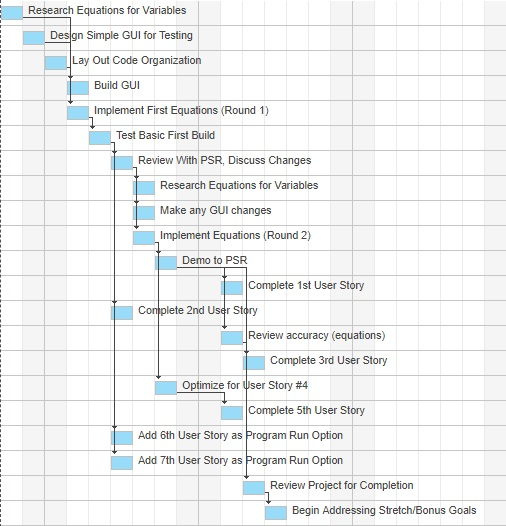
\includegraphics{461Chartcut.jpg}
            \caption{Gantt Chart}
            \label{fig:Gantt}
        \end{figure}
        
    \subsection{Stretch Goals}
    \begin{enumerate}
        \item Record the angle of the sun and the direction the car is facing.
        %\item Include some API to map the elevation changes of the route in detail. 
        \item Include variables from Group 3.
    \end{enumerate}
    
    

\end{singlespace}
\end{document}